\documentclass[journal]{IEEEtran}
\usepackage{amsmath,amssymb,graphicx,booktabs,array,url}
\usepackage[hidelinks]{hyperref}
\hypersetup{pdftitle={Preference-Conditioned Speed and Steering on Rough Ground: Recovery Limits and Ridge Placement},pdfauthor={Anonymous Authors}}
\newcommand{\clip}{\operatorname{clip}}\newcommand{\sat}{\operatorname{sat}}
\newcommand{\E}{\mathbb E}\newcommand{\ind}{\mathbf1}\newcommand{\pos}[1]{[#1]_+}
\title{Preference-Conditioned Speed and Steering on Rough Ground: Recovery Limits and Ridge Placement}
\author{Anonymous Author(s)}
\renewcommand{\topfraction}{0.95}
\renewcommand{\dbltopfraction}{0.95}
\renewcommand{\textfraction}{0.05}
\setcounter{topnumber}{3}\setcounter{dbltopnumber}{3}
\begin{document}\maketitle
\begin{abstract}
Steering generates the lateral reaction that a single-track robot needs both to follow a bend and to arrest a fall. We study a policy that adjusts speed and steering references above a frozen balance controller. Its scalar preference changes the relative costs of speed and path error. In simulation at a requested 2.6~m/s, moving a 10~cm ridge by 0.6~m reversed which endpoint preference completed a 10-s turn in all four paired physical groups. At the first post-crest return of front-wheel load, all eight failing endpoints lacked rear support throughout the initial loaded bout. A constrained nominal roll model shows why steering authority depends on the state reached at recontact. Across two batches of contact records, integrated front and rear wheel moments and the rotating-axis term account for the measured change in vehicle angular momentum with residuals of 1.20\% and 1.03\% by absolute impulse. A 2,112-rollout geometry sweep resolves narrow placement-dependent completion windows. On two held-out layouts a pre-run selector passed the balanced tracking task in 75 of 176 conditions, compared with 70 for the best fixed preference. Fixed preferences passed more conditions under each of the other two tracking specifications.
\end{abstract}
\begin{IEEEkeywords}Single-track robots, reinforcement learning, preference-conditioned control, reference coordination, contact dynamics.\end{IEEEkeywords}

\section{Introduction}
\IEEEPARstart{A}{single}-track robot cannot choose speed, steering, and lean independently. Steering shapes the route and generates balancing reactions. Speed changes lateral acceleration, lean equilibrium, and transient steering response. Accurate path and speed tracking can therefore demand different actions during turns or terrain contact.

We introduce a \emph{preference-conditioned reference policy} (PCRP) above a frozen balance stack. Given $\alpha\in[0,1]$ and recent motion history, it adjusts speed and steering references without changing balance gains. Low $\alpha$ favors the original path; high $\alpha$ favors requested speed. Reference conditioning keeps corrections bounded and smooth. We study the resulting tracking trade-off, lean response, and traversal outcomes.

Classical bicycle dynamics formalize the balance--steering coupling~\cite{meijaard2007}. Reference governors modify commands to prestabilized systems~\cite{garone2017}, and residual reinforcement learning combines analytical control with learned corrections~\cite{johannink2019}. Hierarchical residual path tracking has also been studied for unmanned bicycles~\cite{huo2025}. Our architecture adds a shared preference-conditioned speed/steering interface. Dynamic-weight multiobjective learning~\cite{abels2019} motivates this interface, while the present analysis concerns its physical effect on turns and terrain traversal.

We ask which adjustment remains useful when a wheel unloads in a turn. We connect the preference objective to measured speed and curvature, derive the steering trajectory that minimizes nominal roll at fixed speed, and use wheel-contact impulses to interpret failures that occur near recontact. A frozen selection test then measures how much of the observed preference dependence can be exploited before a run begins.

\begin{figure*}[!t]\centering
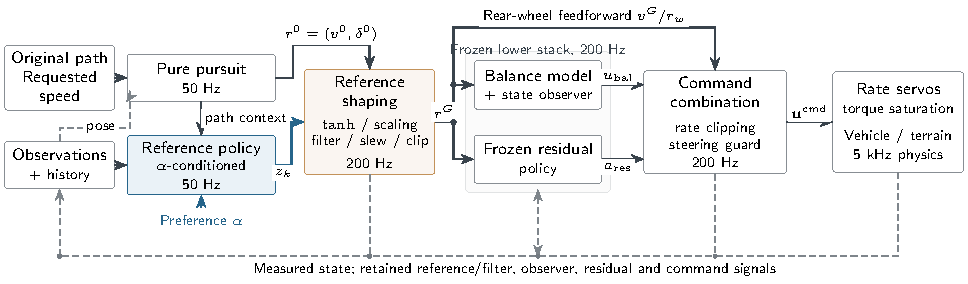
\includegraphics[width=\textwidth]{figures/architecture.pdf}
\caption{Actual signal flow: pure pursuit and the preference-conditioned policy feed reference shaping in parallel. The shaped references drive the frozen balance model, observer, and residual policy. Rear-wheel feedforward bypasses balance feedback and enters command combination directly. Dashed lines carry measurements and stored controller signals; $\alpha$ enters only the reference policy.}
\label{fig:architecture}\end{figure*}
\section{Coupled Vehicle and Control Architecture}
\subsection{Lean--Steering--Speed Coupling}
Let $v,\delta,\phi$ denote body-forward speed, steering angle, and lean. For wheelbase $L$ and caster angle $\beta$, the local low-slip turning relations are
\begin{equation}
 \kappa_v\simeq\frac{\cos\beta}{L}\tan\delta,\qquad
 a_y\simeq v^2\kappa_v,\qquad
 \tan\phi_{\rm eq}\simeq\frac{v^2\kappa_v}{g}.
 \label{eq:steady}
\end{equation}
At a given curvature, retaining speed increases the required lateral acceleration and equilibrium lean. Reducing speed or changing the executed curvature can reduce this demand:
\begin{equation}
 d a_y\simeq2v\kappa_v\,dv+v^2\,d\kappa_v.
 \label{eq:demand}
\end{equation}
The second option changes the executed path, creating the basic tracking trade-off.

The implemented fixed-speed small-angle model also contains a transient steering-rate term:
\begin{equation}
 \ddot\phi=a_4\phi+a_2(v)\delta+a_1(v)\dot\delta+d,
 \label{eq:roll}
\end{equation}
where $d$ is an external generalized lean acceleration. With effective roll inertia $I_e=mh^2+I_{\rm CoM}$,
\begin{align}
 a_4&=mgh/I_e,\nonumber\\
 a_1(v)&=-m\ell hv\cos\beta/(LI_e),\nonumber\\
 a_2(v)&=-(mhv^2-m\ell t_rg)\cos\beta/(LI_e).
 \label{eq:coeff}
\end{align}
Here $h,\ell,t_r$ are center-of-mass height, forward offset, and trail. The nominal controller parameters give $a_4=40.7619$, $a_1=-1.51526v$, and $a_2=1.78195-9.23941v^2$ in SI units. Slowing down reduces turning demand but also reduces the magnitude of steering-rate authority $|a_1|$.

Under small steering angles, substituting $\kappa_v\simeq\delta\cos\beta/L$ into~\eqref{eq:roll} gives both $v^2\kappa_v$ and $v\dot\kappa_v$ terms. An S-bend therefore changes transient steering demand as well as steady turning demand.

\subsection{Preference-Conditioned Reference Policy}
In Fig.~\ref{fig:architecture}, pure pursuit~\cite{coulter1992} maps body-frame preview $(x_\ell,y_\ell)$ to $\kappa^0=2y_\ell/(x_\ell^2+y_\ell^2)$ and $\delta^0=\arctan(L\kappa^0/\cos\beta)$. It publishes slew-limited nominal references for the original path and requested speed $v^{\rm req}$; evaluation retains these original targets.

PCRP has 351 inputs: sixteen 20-field histories, sixteen validity masks, and fifteen context fields. Histories contain body/joint motion, wheel speeds, references, commands, residuals, and observer state; context contains $\alpha$, original-path errors, curvature preview, requested speed, and correction states. Its 128--128--64 ELU actor applies affine modulation~\cite{perez2017} before the last two hidden activations: $h\leftarrow(1+qg)\odot h+qb$, $q=2\alpha-1$.

At each 20~ms middle step, the actor produces a Gaussian latent action during training and its mean during deterministic evaluation:
\begin{equation}
 z_k\sim\mathcal N(\mu_\theta(o_k,\alpha),\Sigma_\theta),
 \qquad a_k=\tanh z_k.
 \label{eq:actor}
\end{equation}
Speed corrections scale negative/positive actions by 1/0.25~m/s; steering uses 0.20~rad. Targets are held for four lower ticks. For channel $i$ and $\Delta_L=0.005$~s,
\begin{align}
 f_{i,j+1}&=e^{-\Delta_L/\tau_i}f_{i,j}
 +(1-e^{-\Delta_L/\tau_i})d_{i,k}^{\rm tar},\nonumber\\
 d_{i,j+1}&=\clip(f_{i,j+1},d_{i,j}-\ell_i^-\Delta_L,
                         d_{i,j}+\ell_i^+\Delta_L),\nonumber\\
 r^G_{i,j+1}&=\clip(r^0_{i,j+1}+d_{i,j+1},r_i^{\min},r_i^{\max}).
 \label{eq:shaping}
\end{align}
Amplitude clipping back-calculates the correction and filter state to the delivered-minus-nominal reference. Table~\ref{tab:interface} gives the numerical interface.

\begin{table}[t]\centering\footnotesize
\caption{Reference interface and inherited training settings.}\label{tab:interface}
\begin{tabular}{@{}ll@{}}\toprule
Reference quantity & Value\\\midrule
Speed / steering correction targets & $[-1,0.25]$ m/s / $\pm0.20$ rad\\
Filter constants $\tau_v,\tau_\delta$ & $0.10,0.08$ s\\
Speed downward / upward slew & $1.0/0.5$ m/s$^2$\\
Steering correction slew & $0.8$ rad/s\\
Delivered $v^G,\delta^G$ bounds & $[1.5,3.5]$ m/s, $\pm0.35$ rad\\
Actor / lower / physics frequency & 50 / 200 / 5000 Hz\\\midrule
Training setting & Value\\\midrule
Environments $\times$ middle steps & $512\times128$ per collection\\
Critic warmup / PPO collections & 2 / 75\\
Discount / GAE / PPO clip & 0.997 / 0.99 / 0.2\\
Max. epochs / minibatches per epoch & 4 / 4\\
Initial actor / critic learning rate & $3\times10^{-5}/3\times10^{-4}$\\\bottomrule
\end{tabular}
\end{table}

\subsection{Frozen Balance Stack and Actuation}
The lower stack combines model-based feedback, an extended-state observer, and a frozen residual policy with 210 inputs, 256--128 hidden widths, and two tanh outputs. Gains use rear-wheel speed $v_w=r_w\omega_r$; task errors use body speed $v$. Equating them in~\eqref{eq:roll} assumes low slip. The observer updates continuously; compensation begins after physical time 3~s.

The lower commands are
\begin{align}
 \dot\delta^{\rm cmd}&=\Pi_{D}\!\left[\clip(u_{\rm bal}+1.5a_{{\rm res},\delta},-3,3)\right],\nonumber\\
 \omega_r^{\rm cmd}&=\clip(v^G/r_w+10a_{{\rm res},r},-60,60),
 \label{eq:commands}
\end{align}
where $\Pi_D$ is the predicted joint-position guard for $|\delta|\leq0.8$~rad. Commands are in rad/s. Velocity servos subsequently apply bounded torque,
$\tau_i=\clip(K_i(u_i^{\rm cmd}-\dot q_i),\tau_i^{\min},\tau_i^{\max})$.
Thus PCRP changes references, and the actual joint response is generated through the lower feedback, servo, and contact dynamics.

\section{Learning Formulation and Reward}
\subsection{Full-State MDP with History-Conditioned Observation}
Define $\mathcal M=(\mathcal X,\mathcal A,P,\rho_0,r_\alpha,\gamma,T)$ with fixed episode context (original path, $v^{\rm req}$, $\alpha$). Full state $\xi_k$ comprises this context, physical/terrain states and parameters, path progress, task clock, controller/observer memory, policy histories, reference filters, and actuators. The two-dimensional latent action $z_k$ advances four lower ticks:
\begin{equation}
 \xi_{k+1}\sim P(\cdot\mid\xi_k,z_k),\qquad
 o_k=\mathcal O(\xi_k),\qquad T=10~\mathrm s.
 \label{eq:mdp}
\end{equation}
The Markov formulation applies to $\xi_k$, not the finite-history observation. In final recovery training, $\rho_0$ samples 320 saved closed-loop states with their route, preference, memory, and task clock preserved. Evaluation uses each protocol's common prepared state. Preference stays fixed within an episode. The actor maximizes
\begin{equation}
 J(\theta)=\E_{\alpha,\rho_0,P,\pi_\theta}
 \left[\sum_{k=0}^{N-1}\gamma^kr_\alpha(\xi_k,z_k)\right],
 \qquad\gamma=0.997.
 \label{eq:objective}
\end{equation}
The critic additionally receives the remaining-task-time fraction. PPO~\cite{schulman2017} uses generalized advantages and the clipped surrogate
\begin{equation}
 L_{\rm clip}=\E_k\min\left(\rho_k\widehat A_k,
 \clip(\rho_k,1-\epsilon,1+\epsilon)\widehat A_k\right),
 \label{eq:ppo}
\end{equation}
Here $\rho_k$ is the current-to-old likelihood ratio and $\epsilon=0.2$. A parent-policy anchor KL term has coefficient 0.05. Table~\ref{tab:interface} records final training settings; evaluation freezes the resulting weights.

\subsection{Implemented Preference Cost}
Errors always refer to the original task: $e_v=v-v^{\rm req}$, signed cross-track error $e_y$, and wrapped path-heading error $e_\psi$. Define $H(x)=x^2$ for $|x|\leq1$ and $H(x)=2|x|-1$ otherwise. The demand gate uses the requested-speed equilibrium lean. With $q(v)=-a_4/a_2(v)$ and original-path curvature $\kappa^{\rm ref}$,
\begin{equation}
\begin{split}
 \phi^{\rm req}_{\rm eq}&=\arctan(L\kappa^{\rm ref}/\cos\beta)/q(v^{\rm req}),\\
 \chi&=\clip((|\phi^{\rm req}_{\rm eq}|-0.18)/0.12,0,1).
\end{split}
 \label{eq:gate}
\end{equation}
Write $B_c(x)=\min(x,c)$ and $[x]_+=\max(x,0)$. Endpoint components are
\begin{align}
 S_0&=(10-9\chi)H(e_v/0.1),&S_1&=10H(e_v/0.1),\nonumber\\
 P_y&=10\big[H(e_y/0.1)+0.5H(e_\psi/0.1)\big],\nonumber\\
 T_0&=20\chi H([|e_y|-0.1]_+/0.1),\nonumber\\
 T_1&=20\chi H([|e_v|-0.05]_+/0.1).
 \label{eq:endpoints}
\end{align}
Physical divisors are respectively in m/s, m, and rad. The effective preference cost is
\begin{equation}
\begin{split}
 C_\alpha={}&(1-\alpha)B_{200}(S_0)+\alpha B_{200}(S_1)\\
 &+(1-0.9\alpha)B_{200}(P_y)\\
 &+(1-\alpha)B_{400}(T_0)+\alpha B_{400}(T_1).
\end{split}\label{eq:prefcost}
\end{equation}
Each endpoint is capped before mixing. At $\chi=1$ and below the caps, speed and path weights are $1+9\alpha$ and $10-9\alpha$.

\begin{table}[t]\centering\footnotesize
\caption{Common costs, each capped separately. $\phi_{\rm pk}$ is peak absolute lean during a lower tick.}\label{tab:common}
\begin{tabular}{@{}p{18mm}p{48mm}r@{}}\toprule
Term & Uncapped cost & Cap\\\midrule
Lean & $80H([\phi_{\rm pk}-.26]_+/.04)$ & 1800\\
Working lean & $240H([\phi_{\rm pk}-.30]_+/.02)$ & 6000\\
Lean rate & $H([|\omega|-.8]_+/.8)$ & 40\\
Overspeed & $2H([e_v-.05]_+/.1)$ & 160\\
Low speed & $4H([1.5-v]_+/.2)$ & 160\\
Offset & $.02[(d_v/1)^2+(d_\delta/.2)^2]$ & .2\\
Offset rate & $.03[(\dot d_v/1)^2+(\dot d_\delta/.4)^2]$ & 20\\\bottomrule
\end{tabular}
\end{table}

Table~\ref{tab:common} gives the common costs in SI units. With $C_{c,j}$ containing its first six terms, a normal 20~ms step has reward
\begin{equation}
\begin{split}
 r_k={}&-0.1\Delta_L\sum_{j=1}^4(C_{\alpha,j}+C_{c,j})\\
     &-0.1\Delta_M C_{\dot d,k},\qquad\Delta_M=.02~\mathrm s.
\end{split}
 \label{eq:reward}
\end{equation}
The rate cost uses the net applied offset change over the middle step and is counted once. On a newly failing transition, the entire reward is replaced by
\begin{equation}
 r_k^{\rm fail}=-5-0.1\Delta_M C_{\max}
 \frac{1-\gamma^{N_k}}{1-\gamma},\qquad C_{\max}=8980.2,
 \label{eq:terminal}
\end{equation}
where $N_k$ includes the failing interval and the remaining original-task intervals. Subsequent inactive steps receive zero.

For any fixed trajectory and termination, $F_\alpha=(1-\alpha)F_0+\alpha F_1$: increasing $\alpha$ shifts the objective toward speed tracking. Actual tracking and traversal determine the resulting behavior.

\section{Physical Interpretation and a Common Evaluation Rule}
\subsection{Preference and Measurable Turning Demand}
A preference changes the reward weights, then changes the speed and steering references through the learned policy. Let $v_0$ be requested speed, $v$ measured speed, $K=|\kappa^{\rm ref}|$, and $\kappa$ the executed curvature signed in the original bend direction. For smooth, low-slip turning, the demand-reduction proxy is
\begin{equation}
\begin{split}
 D&=v_0^2K-v^2\kappa,\\
 D_{\rm lin}&=2v_0K(v_0-v)+v_0^2(K-\kappa).
\end{split}
 \label{eq:allocation}
\end{equation}
The first-order terms distinguish slowdown from curvature change and may have either sign. We use measured curvature, not outward displacement, for this check.

For the base tracking terms at fixed $\chi$, in their quadratic and uncapped region, the path-to-speed weight ratio is
\begin{equation}
 r(\alpha)=\frac{10-9\alpha}{10-9\chi+9\chi\alpha},\qquad
 \frac{\partial r}{\partial\alpha}=
 \frac{-9(10+\chi)}{(10-9\chi+9\chi\alpha)^2}<0.
 \label{eq:weights}
\end{equation}
Increasing $\alpha$ therefore makes speed error more costly relative to path error. Combined with~\eqref{eq:allocation}, this motivates a testable direction: less slowdown and more change in executed curvature. The bend and error-plane results test this direction; the weight relation is not an exact optimizer of the full task.

\subsection{Endpoint objectives and constrained roll recovery}
For a policy $\pi$, let $F_0(\pi)$ and $F_1(\pi)$ include all gated tracking, common and terminal costs under the two endpoint preferences. For any feasible policies minimizing $(1-\alpha)F_0+\alpha F_1$ exactly at $a<b$, the two optimality inequalities give
$ (1-a)\Delta F_0+a\Delta F_1\geq0$ and
$ (1-b)\Delta F_0+b\Delta F_1\leq0$, with differences evaluated from the first policy to the second. Thus $\Delta F_0\geq0$ and $\Delta F_1\leq0$. The learned actor is approximate, and individual tracking errors omit shared costs.

Fix speed $v\geq0.5$~m/s in the nominal model and set $\lambda=\sqrt{a_4}$. After integrating the steering-rate input by parts, the contribution of the steering history to roll at time $T$ is
\begin{equation}
\int_0^T \left[a_1\cosh(\lambda(T-t))+
  \frac{a_2}{\lambda}\sinh(\lambda(T-t))\right]\delta(t)\,dt .
\end{equation}
The remaining terms depend only on the initial state. Both coefficients are negative over this speed range. Under $|\dot\delta|\le U$ and $|\delta|\le D$, the greatest feasible steering angle at every instant is $\min(D,\delta_0+Ut)$. This single feasible history minimizes roll for every horizon; $\max(-D,\delta_0-Ut)$ gives the upper roll envelope. Crossing the positive roll limit even on the lower envelope certifies unavoidable crossing in this frozen nominal model. The corresponding statement applies to the negative limit using the upper envelope. Contact and actuator dynamics can shift the physical crossing time.

\subsection{Wheel support and the roll impulse budget}
Let $L_C$ denote whole-vehicle angular momentum about its center of mass. We reconstruct it from the rotational and orbital momenta of six rigid bodies. For the recorded wheel-only contact windows, let $e$ be a body-fixed roll axis expressed in world coordinates and $\Omega$ the chassis angular velocity. The projected change satisfies
\begin{equation}
\Delta(e^\top L_C)=\int e^\top(\tau_{f,C}+\tau_{r,C})\,dt+
\int (\Omega\times e)^\top L_C\,dt .
\end{equation}
Uniform gravity has zero moment about the center of mass. A fully unloaded front wheel contributes no ground moment even while the steering joint moves. The second integral retains the change in projection axis during the impact.
\subsection{An Obstacle Is Encountered at a Particular Turning Phase}
Figure~\ref{fig:terrain} uses the same smooth 90-degree left-turn route and ridge shape in both trials. The obstacle center moves from route progress $s_c=3.9$ to $4.5$~m. Both centers lie on the constant-curvature portion, where the archived path has $\kappa^{\rm ref}=1/1.8$~m$^{-1}$. The center heading changes by $\Delta\psi^{\rm ref}=0.6/1.8=0.333$~rad ($19.1^\circ$), while the local curvature remains identical. The shift changes encounter phase and reference orientation, not turn sharpness, and is not a translation under an unchanged vehicle pose.

PCRP changes speed and steering together. Its endpoint preferences consequently reach these two placements with different speeds, lean, and steering states. Equation~\eqref{eq:roll} shows why these quantities matter: the steering-angle and steering-rate terms depend on speed, and their signs can oppose or reinforce the current roll motion. Both preferences retain the same $\pm3$~rad/s steering-command and $\pm1$~N\,m steering-torque limits. Changing $\alpha$ changes the reached state, not hardware authority.

Ridge length changes the geometric excitation as well as encounter timing. On the analytic centerline, write $q=s-s_c$ and $z_g=h_r\cos^2(\pi q/\ell_r)$ for $|q|\leq\ell_r/2$, where $h_r$ and $\ell_r$ are ridge height and length. Then
\begin{equation}
 \max|z'_g|=\frac{\pi h_r}{\ell_r},\qquad
 \max|z''_g|=\frac{2\pi^2h_r}{\ell_r^2}.
 \label{eq:ridgeprofile}
\end{equation}
Along that profile, $\ddot z_g=z''_g\dot q^2+z'_g\ddot q$. At the same constant profile speed, increasing $\ell_r$ from 0.8 to 1.2~m reduces the peak geometric second-derivative term to $4/9$. This is a continuous terrain-profile scale, not the robot's measured lean acceleration; the simulator samples and quantizes the height field. We test whether the gentler profiles expand completion, while the recorded vehicle states explain why a preference can fail at one placement and complete at another.

\subsection{One Traversal Criterion, Separate Tracking Measures}
We use one fixed physical-completion criterion for the endpoint comparison in Fig.~\ref{fig:terrainresults}:
\begin{equation}
 C_{10}=\ind_{\{\text{the complete 10-s rollout has no termination}\}}.
 \label{eq:completion}
\end{equation}
Terminations include $|\phi|>0.70$~rad, contact failure, and follower-domain exit. With path preview $p_\ell$, vehicle position $p$, and heading $\psi$, the follower margins are
\begin{equation}
\begin{split}
 m_x&=[\cos\psi,\sin\psi](p_\ell-p)-0.05,\\
 m_\psi&=\pi/2-|\operatorname{wrap}(\psi-\psi_{\rm path})|.
\end{split}
 \label{eq:domain}
\end{equation}
Failure types are counted separately; completion does not imply accurate tracking.

Tracking errors remain relative to the original route and requested speed:
\begin{equation}
 E_p=\max_t|e_y(t)|,\qquad
 E_v=\sqrt{\frac{1}{n}\sum_{j=1}^n(v_j-v^{\rm req})^2}.
 \label{eq:metrics}
\end{equation}
Final-window tracking $H$ requires every 200~Hz sample in the last second to satisfy $|e_y|\leq0.10$~m, $|e_\psi|\leq0.05$~rad, and $|e_v|\leq0.10$~m/s. The separate, fixed balanced tracking criterion is
\begin{equation}
 S_C=C_{10}\ind_H\ind_{\{E_p\leq0.40\,\mathrm m\}}
                    \ind_{\{E_v\leq0.15\,\mathrm{m/s}\}}.
 \label{eq:success}
\end{equation}
Neither criterion changes with preference or terrain. The main endpoint figure uses $C_{10}$ throughout; $S_C$ is reported separately so that completion is not mistaken for tracking-task success.

\section{Simulation Study}
\subsection{Experimental Conditions and Evaluation Order}
Table~\ref{tab:experiments} separates route geometry, terrain, and imposed lateral pulses. We report historical preference-dependent bending motion and examine the ridge-placement reversal and its recorded states. A one-factor study tests the wider role of position, slope length, and relative geometry. The original terrain scan supplies the seven terrain-height comparisons. All comparisons use the same frozen middle actor. The terrain scans and error-plane runs share the same balance stack. Historical smooth-bend comparisons used separately archived execution settings and are reported as supporting evidence. Within each condition, route, speed request, saved initial state, physical parameters, and pulse schedule are matched across preferences.

\begin{table}[t]\centering\footnotesize
\caption{Experimental conditions and their roles. ``Pulse'' denotes an imposed lateral force, in addition to wheel--ground contact.}\label{tab:experiments}
\begin{tabular}{@{}p{17mm}p{35mm}p{28mm}@{}}\toprule
Study & Ground and pulse condition & Main question\\\midrule
Bends & Flat; unforced single bend and pulsed S-bend & How does preference change the trajectory?\\
Error plane & Flat or 20/40/60~mm ridge; no pulse & How do tracking errors trade off?\\
Terrain scan & 4/6/8/10~cm ridge or 5/10/20~mm gravel; no pulse & Which preferences complete and track?\\
Layout pair & 10~cm ridge centered at 3.9/4.5~m; no pulse & Does placement reverse endpoint completion?\\
Geometry scan & 10~cm ridge and matched flat controls; no pulse & Which preference windows persist across geometry?\\\bottomrule
\end{tabular}
\end{table}

The 20-condition error-plane study crosses the four surfaces in Table~\ref{tab:experiments} with speeds 1.5, 1.8, 2.0, 2.3, and 2.6~m/s. Five preferences and five physical groups share a saved 2.3~m/s warm initial state and within-group RMSE window.

The terrain study follows a smooth 90-degree left turn with a 1.8~m constant-curvature radius. Its 22 conditions combine four ridge heights with speeds 1.8, 2.1, 2.3, and 2.6~m/s, and three gravel heights with speeds 2.3 and 2.6~m/s. Figure~\ref{fig:terrain} locates the two ridge placements on the actual route. The oblique ridge has a 0.8~m longitudinal profile, 0.8~m half-width, and obliquity coefficient 0.25. Gravel occupies route progress 3--7~m. Stone centers are generated at 24/m$^2$ before lateral compression by 0.25, giving a 0.20~m center half-width; radii are 0.055--0.08~m.

\begin{figure*}[!t]\centering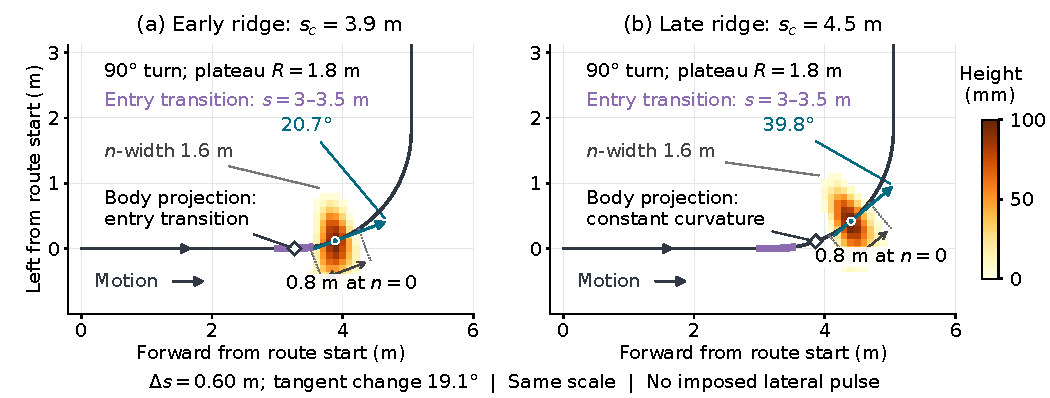
\includegraphics[width=\textwidth]{figures/terrain_overview.pdf}
\caption{Two placements of the same 10~cm ridge on the same recorded left-turn route. Axes and height scales are identical. The ridge center moves by 0.6~m along the path, from $s_c=3.9$ to $4.5$~m, while route heading at the center changes from $20.69^\circ$ to $39.78^\circ$. Purple marks the curvature-transition segment. Diamonds mark the mean chassis projection when the front-wheel center crosses the upstream boundary, not the actual chassis XY. The panels are alternative layouts.}
\label{fig:terrain}\end{figure*}

The original scan uses thirteen preferences plus a no-correction baseline, four physical groups, and two executions: 2464 rollouts. Groups fix friction, mass scale, servo gain, and steering offset across preferences. A 2112-rollout layout test changes ridge centers to 3.9/4.5~m and gravel arrangements, using four further groups with five preferences, baseline, and selection lanes. Figure~\ref{fig:terrainresults} uses only fixed preferences.

The post-layout one-factor development study adds 2112 rollouts: 44 cells, eight physical groups, and five preferences plus baseline. It tests 13 positions, seven lengths at two positions, five wheelbase scales with flat controls, five obliquities, and three whole-scene rotations. Shared baseline cells count once. Height, speed request, and controller remain fixed at 0.10~m, 2.6~m/s, and the original parameters. Four groups reuse earlier parameter sets; four extend the range. The studies are not pooled: repeated execution preserves the endpoint reversal but changes some intermediate counts. These are parameter blocks, not training seeds or independent selector tests.

\subsection{Metrics Used in Each Test}
Bends use speed, curvature, and outward displacement; the error plane uses matched-window RMSE. Completion figures use $C_{10}$ with all failures in the denominator. Separate $E_p,E_v,S_C$ scores retain the original targets; the robot continues after crossing the goal.

\subsection{Bending Motion and the Speed--Path Exchange}
In the historical flat-bend study, recorded speed and curvature allow a direct check of~\eqref{eq:allocation}. Curvature is computed from the 200~Hz XY records using a 205~ms third-order Savitzky--Golay derivative window. In the 40-run five-preference and 96-run three-preference unforced batches, the mean absolute first-order demand error is 0.147 and 0.089~m/s$^2$, respectively, over sustained-curvature segments. Increasing preference raises turning speed and reduces the slowdown contribution in all 96 adjacent-preference comparisons; signed outward deviation increases in 94. These observations support the direction motivated by~\eqref{eq:weights}, while the measured curvature, rather than outward displacement alone, supplies the demand decomposition.

Figure~\ref{fig:tradeoff} then compares tracking errors at a common requested speed of 2.6~m/s. On flat ground and 20-/40-mm ridges, increasing $\alpha$ reduces speed RMSE and raises position RMSE. Across the full 20-condition set, 41 of 80 adjacent comparisons follow that ordering; terrain contact and transient motion can change it.

\begin{figure*}[!t]\centering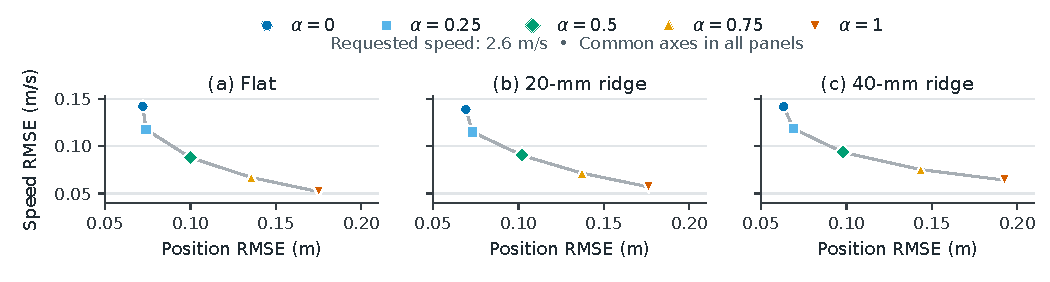
\includegraphics[width=.98\textwidth]{figures/speed_position_tradeoff.pdf}
\caption{Selected speed--position trade-offs at 2.6~m/s on flat ground and 20-/40-mm ridges, using common axes. Each point is the square root of the mean of MSEs from five physical groups over a common window. Lines join adjacent preferences.}
\label{fig:tradeoff}\end{figure*}

\subsection{Endpoint Reversal Under One Completion Standard}
Figure~\ref{fig:ridgepaths} follows all six vehicles until their individual endpoints. The other physical groups enter the counts below.
\begin{figure}[!t]\centering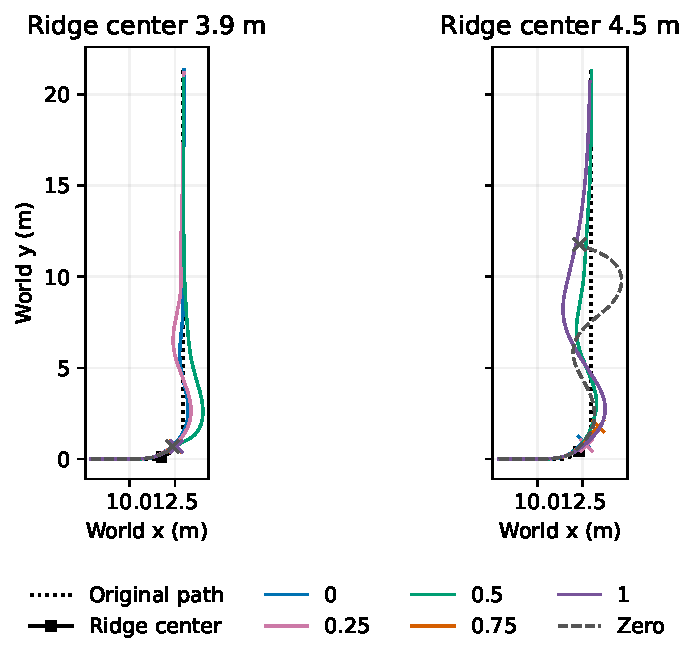
\includegraphics[width=\columnwidth]{figures/ridge_paths.pdf}
\caption{Actual and original XY in physical group 401, at 2.6~m/s without a pulse. Colors identify the five fixed preferences; Zero retains the frozen lower stack. Crosses mark early termination. Both panels have equal metric aspect.}
\label{fig:ridgepaths}\end{figure}

Figure~\ref{fig:terrainresults} compares the same 10~cm ridge at the same 2.6~m/s speed request, with its center placed at $s=3.9$ or $4.5$~m. Each preference uses the same four physical-parameter groups within a layout. At 3.9~m, $\alpha=0$ completes all four runs and $\alpha=1$ completes none; at 4.5~m, these counts reverse. All eight failed endpoint runs terminate at the lean limit, rather than at the follower-domain boundary.

\begin{figure*}[!t]\centering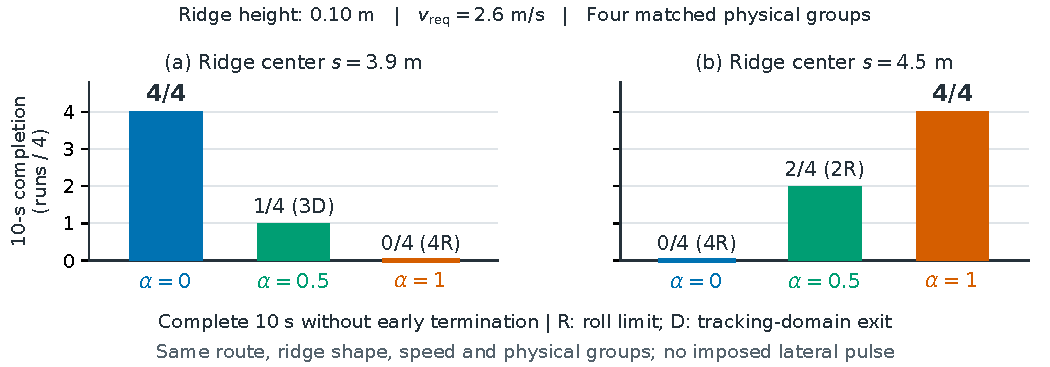
\includegraphics[width=.89\textwidth]{figures/terrain_tasks.pdf}
\caption{Endpoint advantage reverses with ridge placement under one unchanged criterion: completing 10~s without termination. Both panels use a 10~cm ridge, the same smooth left-turn route, a 2.6~m/s request, no imposed pulse, and four matched physical groups. Only the ridge-center position changes between panels. All four losing endpoint runs in each panel terminate at the lean limit. Counts are completed runs out of four, not Task-C successes.}
\label{fig:terrainresults}\end{figure*}

\begin{figure*}[!t]\centering
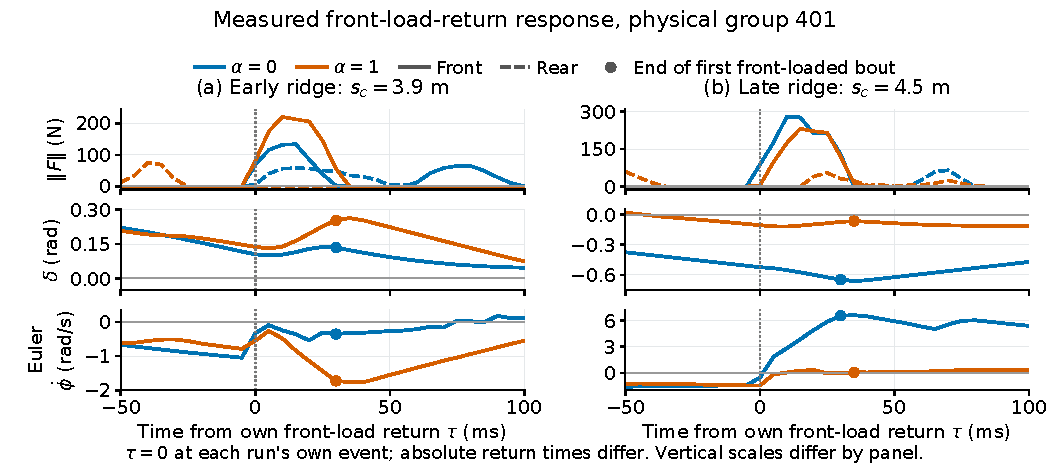
\includegraphics[width=.96\textwidth]{figures/endpoint_states.pdf}
\caption{Front-wheel load-return events in physical group 401. Blue/orange: $\alpha=0/1$; solid/dashed forces: front/rear. Each run uses its own post-peak front-load return as $\tau=0$: 1.640/1.625~s at the early ridge and 1.945/1.875~s at the late ridge. Dots mark the bout end. All plotted values are unsmoothed 200~Hz records.}
\label{fig:states}\end{figure*}

\begin{figure*}[!t]\centering
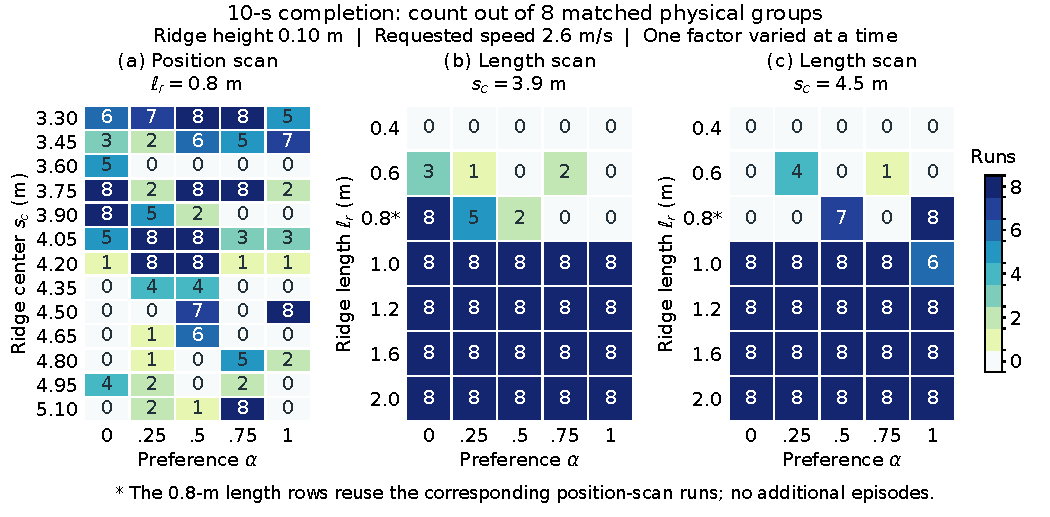
\includegraphics[width=\textwidth]{figures/geometry_windows.pdf}
\caption{Complete one-factor grids under $C_{10}$. Entries count 10-s completions out of eight matched groups. (a) All 13 positions with length 0.8~m. (b,c) All seven lengths at the two positions. The 0.8~m rows reuse (a), not additional trials. Height and requested speed stay fixed at 0.10~m and 2.6~m/s.}
\label{fig:oat}\end{figure*}

Across all five preferences, completion is $[4,3,1,0,0]$ at 3.9~m and $[0,0,2,0,4]$ at 4.5~m. Thus each endpoint is uniquely best in its layout. These examples were found by screening all 44 terrain--speed--layout cells. The middle preference's three early-layout failures are domain exits; its two late-layout failures are lean-limit terminations.

Completion and tracking still differ. The completing low endpoint reaches final-window tracking in 4/4 runs and Task C in 1/4; the completing high endpoint reaches them in 2/4 and 0/4. The reversal is therefore in physical completion, not tracking-task success.

\subsection{Arrival State and Wheel-Support Sequence}
Table~\ref{tab:arrival} records the first 200~Hz sample at or beyond the front-wheel-center upstream crossing, $s_f-s_c-0.25n_f=-0.4$~m. This geometric section is not first tire contact. The chassis projection is then at $s=3.261$--$3.271$~m for the early ridge, within the $3.0$--$3.5$~m curvature transition, but at $3.871$--$3.878$~m for the late ridge, on the constant-curvature segment. Thus identical center curvature does not imply identical encounter phase. At the late ridge, low-preference runs arrive slower and with larger steering than their early-ridge counterparts; high-preference runs also change lean and steering.

\begin{table}[t]\centering\footnotesize
\caption{Measured state at the front-wheel-center upstream crossing, averaged over four physical groups. $\kappa_b^{\rm ref}$ is reference curvature at the chassis projection, not at the ridge center.}\label{tab:arrival}
\begin{tabular}{@{}lcrrrr@{}}\toprule
$s_c$ (m) & $\alpha$ & $v$ (m/s) & $\phi$ (rad) & $\kappa_b^{\rm ref}$ (m$^{-1}$) & $\delta$ (rad)\\\midrule
3.9 & 0 & 2.184 & 0.187 & 0.301 & 0.143\\
3.9 & 1 & 2.498 & 0.162 & 0.303 & 0.090\\
4.5 & 0 & 2.088 & 0.227 & 0.556 & 0.214\\
4.5 & 1 & 2.418 & 0.239 & 0.556 & 0.166\\\bottomrule
\end{tabular}
\end{table}

The ensuing wheel-support sequence distinguishes the endpoint outcomes. We identify the first front-wheel load return after its center passes the profile peak: front force rises above 1~N after ten consecutive 5-ms samples below 1~N. The immediate loaded bout contains six to eight samples. In all eight failing endpoints, the rear-wheel force is zero at every sample in this bout. In all eight completing endpoints, the rear wheel also carries load in 50--100\% of those samples. Figure~\ref{fig:states} shows these events for physical group 401 alongside actual steering and roll rate.



At the early ridge, the high-preference vehicle reloads its front wheel without rear support. From the sample before load return to the bout end, its roll rate changes from $-0.79$ to $-1.72$~rad/s in the illustrated run. The low-preference vehicle has overlapping front/rear support and decreasing negative roll-rate magnitude. This contrast holds in all four groups.

At the late ridge, group 401's low-preference run has $\delta=-0.509$~rad just before front-load return. Roll rate then changes from $-1.41$ to $+6.54$~rad/s while steering remains negative. Positive steering-command saturation cannot return the joint through zero before the lean limit. The paired high-preference run starts its event at $\delta=-0.093$~rad, obtains rear support, and ends near zero roll rate. All four low-preference runs show the same roll reversal with negative steering.

The sign structure of~\eqref{eq:roll} helps interpret the late-ridge response: once roll rate is positive while $\delta<0$, the term $a_2(v)\delta$ promotes the current roll direction, and steering cannot reverse instantaneously. The slower endpoint wins at the early ridge and loses at the late ridge. Preference must match terrain placement and task: the early ridge favors the low endpoint for completion, the late ridge the high endpoint.

\subsection{Recovery envelope and measured contact impulses}
In a separate central-ridge run at 2.6~m/s, the speed-priority vehicle reached $-24.30^\circ$ roll and $-534.13^\circ$/s roll rate at 1.940~s. Even the most favorable admissible steering history crossed the negative limit 29.25~ms later in the nominal model. The simulated vehicle terminated 30~ms after that sampled state. Starting 40~ms earlier gave 131~ms in the model and 70~ms in the simulator. The agreement close to failure depends on where the initial state is taken. Across 36 discretized linear programs, the greatest endpoint difference from the discrete envelope was $3.20\times10^{-14}$~rad.

In two batches of 1,697 and 2,042 wheel-contact windows, we computed the angular-momentum change from body motion and the two impulse terms from contact data and axis motion. Summed absolute residual divided by the sum of absolute budget terms was 1.20\% and 1.03\%, respectively. In the failing low-preference runs, front-wheel support vanished and adverse rear-wheel torque dominated the final 100~ms. This diagnosis is conditional on the measured state and contact sequence.
\subsection{One-Factor Geometry Study}
Figure~\ref{fig:oat} extends the endpoint reversal to eight matched groups and shows all tested positions and lengths under $C_{10}$. Moving farther to 4.65~m reduces high-endpoint completion to 0/8 while the middle preference completes 6/8. Thus the favorable window does not shift monotonically toward higher $\alpha$ through the turn.



Gentler profiles expand this range. At lengths 0.4, 0.8, and 1.2~m, completion across both positions rises from 0/80 through 30/80 to 80/80. Archived summaries give corresponding mean longest front-wheel unloading bouts of 0.397, 0.275, and 0.109~s, using force magnitude below 0.1~N within each actual lifetime. This co-variation supports the profile scaling in~\eqref{eq:ridgeprofile}, not an unloading-duration failure rule. All preferences complete from 1.2~m and achieve final-window tracking from 1.6~m. At the 0.8~m late ridge, high-endpoint completion is 8/8 but final-window tracking only 4/8. Across all 352 high-endpoint runs, $S_C=0$.

At center 4.2~m and length 0.8~m, obliquities $-0.5$, $+0.25$, and $+0.5$ yield 0/40, 19/40, and 22/40 completions. Whole-scene rotations of $0^\circ$, $45^\circ$, and $90^\circ$ retain 8/8 completion and final-window tracking for $\alpha=0.25,0.5$, despite changes at edge preferences. Relative geometry matters; absolute world heading alone is not a selection rule.

With the controller frozen, wheelbase scales 1.0, 1.1, and 1.2 yield 30/80, 11/80, and 1/80 ridge completions, despite 40/40 completion and final-window tracking on flat ground. The front-assembly displacement changes aggregate mass distribution as well as wheel spacing. Longer wheelbase is therefore not an automatic improvement under the original controller.

\subsection{Other Terrain and Channel Conditions}
The original terrain scan also contains an internal preference window: on the 10~cm ridge at 2.6~m/s, each tested $\alpha\in\{0.2,0.25,0.3,0.4,0.5,0.6\}$ completes 8/8 runs, while both endpoints complete none. Its layout and physical groups differ from Fig.~\ref{fig:terrainresults}. On 20~mm gravel, the representative preferences $0,0.5,1$ complete only 1/16, 4/16, and 3/16, with no Task-C successes.

\begin{table}[t]\centering\footnotesize
\caption{Original-layout counts under two separately defined, unchanged criteria. Columns within each group are $\alpha=0,0.5,1$. Ridge rows pool four speeds; gravel rows pool two. Each speed has four physical groups and two executions.}\label{tab:terraincounts}
\begin{tabular}{@{}lrrrrrrr@{}}\toprule
& &\multicolumn{3}{c}{$C_{10}$ completion}&\multicolumn{3}{c}{$S_C$ tracking}\\
Terrain & $n$ & $0$ & $.5$ & $1$ & $0$ & $.5$ & $1$\\\midrule
Ridge 4 cm &32&32&32&32&32&32&22\\
Ridge 6 cm &32&32&32&32&29&23&1\\
Ridge 8 cm &32&32&25&28&5&2&7\\
Ridge 10 cm &32&24&32&17&1&9&0\\
Gravel 5 mm &16&16&16&16&10&10&3\\
Gravel 10 mm &16&8&13&16&0&1&2\\
Gravel 20 mm &16&1&4&3&0&0&0\\\bottomrule
\end{tabular}
\end{table}

Channel ablation uses $\alpha=0.5$, two speeds, and three physical groups. On the 10~cm ridge, joint corrections reach final-window tracking in 6/6 runs, versus 1/6 for steering alone and 0/6 for speed alone. On 10~mm gravel, steering alone instead exceeds joint correction (5/6 versus 3/6). Both the useful preference and the useful balance of correction channels depend on the condition.

\section{What the preference selector can predict}
The pre-run selector used terrain family, height, requested speed and the tracking specification. Its decision was frozen before testing on two new layouts and four further physical groups. Each task required completion, final hold and bounds on peak lateral error and speed RMSE. The bound pairs (m, m/s) were $(0.30,0.20)$, $(0.60,0.10)$ and $(0.40,0.15)$ for A, B and C.

\begin{table}[t]\centering
\caption{Passing conditions on new layouts. Each cell has denominator 176. Fixed columns use the same preference in every condition.}
\begin{tabular}{lrrrrrr}\toprule
Task & 0 & .25 & .5 & .75 & 1 & Selector\\\midrule
A & 68 & 56 & 47 & 23 & 8 & 64\\
B & 0 & 24 & 63 & 71 & 62 & 64\\
C & 70 & 64 & 63 & 44 & 32 & 75\\\bottomrule
\end{tabular}\end{table}
On C, the selector gained 15 passes and lost 10 relative to fixed zero preference. Crossed resampling of layouts and physical groups gave a descriptive 95\% interval of $[-3.41,8.52]$ percentage points for the net gain. Its 9/48 gravel passes also fell short of 17/48 for the middle preference. Ridge location was absent from the selector inputs. At fixed height and requested speed, the selector therefore assigned the same setting to placements with different endpoint outcomes.

The experiments used one trained middle policy. Physical groups measure sensitivity to the sampled vehicle and contact parameters. A separate natural switching study found that none of 60 prefix groups met its predeclared common-state check at the switch, so it cannot isolate the effect of changing the post-entry preference. A test of online selection requires matched entry states, a causal post-ridge trigger and layouts reserved before tuning.

\section{Conclusion}
A preference-conditioned policy can change the approach to the same obstacle enough to reverse which endpoint completes the turn. The contact records identify a short interval in which a front wheel reloads while rear support is absent, and the steering envelope quantifies how little recovery authority remains in some of the resulting states. These observations explain why a setting chosen from height and requested speed alone transfers unevenly across placements and tracking tasks.
\begin{thebibliography}{8}
\bibitem{meijaard2007} J. P. Meijaard, J. M. Papadopoulos, A. Ruina, and A. L. Schwab, ``Linearized dynamics equations for the balance and steer of a bicycle: A benchmark and review,'' \emph{Proc. R. Soc. A}, vol. 463, no. 2084, pp. 1955--1982, 2007, doi: 10.1098/rspa.2007.1857.
\bibitem{garone2017} E. Garone, S. Di Cairano, and I. Kolmanovsky, ``Reference and command governors for systems with constraints: A survey on theory and applications,'' \emph{Automatica}, vol. 75, pp. 306--328, 2017, doi: 10.1016/j.automatica.2016.08.013.
\bibitem{johannink2019} T. Johannink \emph{et al.}, ``Residual reinforcement learning for robot control,'' in \emph{Proc. IEEE Int. Conf. Robotics and Automation}, 2019, pp. 6023--6029, doi: 10.1109/ICRA.2019.8794127.
\bibitem{huo2025} B. Huo, L. Yu, Y. Liu, and Z. Chen, ``Hierarchical residual reinforcement learning based path tracking control method for unmanned bicycle,'' \emph{Robotics and Autonomous Systems}, vol. 190, Art. no. 104996, 2025, doi: 10.1016/j.robot.2025.104996.
\bibitem{abels2019} A. Abels, D. Roijers, T. Lenaerts, A. Now\'{e}, and D. Steckelmacher, ``Dynamic weights in multi-objective deep reinforcement learning,'' in \emph{Proc. 36th Int. Conf. Machine Learning}, PMLR, vol. 97, pp. 11--20, 2019.
\bibitem{coulter1992} R. C. Coulter, ``Implementation of the pure pursuit path tracking algorithm,'' Carnegie Mellon University, Tech. Rep. CMU-RI-TR-92-01, 1992.
\bibitem{perez2017} E. Perez, F. Strub, H. de Vries, V. Dumoulin, and A. Courville, ``FiLM: Visual reasoning with a general conditioning layer,'' arXiv:1709.07871, 2017, presented at AAAI 2018.
\bibitem{schulman2017} J. Schulman, F. Wolski, P. Dhariwal, A. Radford, and O. Klimov, ``Proximal policy optimization algorithms,'' arXiv:1707.06347, 2017.
\end{thebibliography}

\end{document}
